\section{Power Distribution Assembly}
\resetassemblysteps

To complete the set up for the encoders, power must first be distributed
to the motors and encoders.

\begin{partsbox}
\begin{minipage}[t]{\linewidth}
\vspace{0pt}
\begin{itemize}
\item
  4 \protect\hyperlink{mk5i-swerve-module-assembly}{Assembled Swerve
  modules}
\item
  1 \href{https://store.ctr-electronics.com/products/pdp-2}{PDP 2.0} --
  \href{https://ctre.download/files/user-manual/PDP\%202.0\%20User's\%20Guide.pdf}{User
  Guide} --
  \href{https://github.com/CrossTheRoadElec/Device-CADs/raw/refs/heads/master/PDP2.0_CAD/PDP\%202.0\%20CAD.zip}{CAD
  File}
\item
  1
  \href{https://store.ctr-electronics.com/products/120-amp-breaker?pr_prod_strat=e5_desc\&pr_rec_id=6ce3ee740\&pr_rec_pid=8010746855597\&pr_ref_pid=8358474383533\&pr_seq=uniform}{120
  Amp Circuit Breaker}
\item
  8
  \href{https://store.ctr-electronics.com/products/auto-resetting-ato-breakers?pr_prod_strat=jac\&pr_rec_id=096140681\&pr_rec_pid=8358474383533\&pr_ref_pid=7922412847277\&pr_seq=uniform}{40
  Amp Auto-Reset Breakers} --
  \href{https://ctre.download/files/datasheet/CTRE\%20Breaker\%20Datasheet.pdf}{Data
  Sheet} - \href{https://ctre.download/cad/25-656640.step}{CAD}
\item
  4
  \href{https://store.ctr-electronics.com/products/auto-resetting-ato-breakers?variant=45044982644909}{10
  Amp Auto-Reset Breakers} --
  \href{https://ctre.download/files/datasheet/CTRE\%20Breaker\%20Datasheet.pdf}{Data
  Sheet} - \href{https://ctre.download/cad/25-656610.step}{CAD}
\item
  1
  \href{https://andymark.com/products/mk-es17-12-12v-sla-battery-set-of-2}{MK
  ES17-12 12V SLA Battery} --
  \href{https://s3.amazonaws.com/docusync-files/cacc1eb873bfa1d6bda7b8a738560a16992dd936cd4f6e119a512326d85e2759/am-0844\%20ES17-12\%20User\%20Guide.pdf}{User
  Guide}
\item
  1
  \href{https://andymark.com/products/6-gauge-12-inch-battery-cable?pr_prod_strat=jac\&pr_rec_id=099dfc460\&pr_rec_pid=8263871365292\&pr_ref_pid=8263859503276\&pr_seq=uniform}{6
  Gauge 12'' Battery Cable} --
  \href{https://s3.amazonaws.com/docusync-files/728a9a02b6997b608f834bc0d313a6780025a444f59a5906b091c7c41b2a654c/am-0009\%20Replacing\%20Wires\%20in\%20a\%20SB50\%20Connector_.pdf}{Replacing
  Wire Guide} -
  \href{https://s3.amazonaws.com/docusync-files/acfa0911a51f1f9ec7a07c8cdab5bda8519f734912ab19342f1d5b9b948663ea/am-4483\%206\%20Gauge\%2012\%20Inch\%20Battery\%20Cable,\%20Flexible\%20EPDM.pdf}{Drawing}
\item
  1
  \href{https://andymark.com/products/robot-power-cable-kit-custom-lengths-up-to-36-in?variant=44493418758316}{6
  Gauge 16'' 9'' Custom Power Cable} (Includes the 120 Amp breaker)
\end{itemize}
\end{minipage}
\end{partsbox}

\assemblystep{Assemble the Power Distribution Panel}
Assemble the Power Distribution Panel (PDP) with the 120A breaker and
power cables as shown.

\begin{figure}[H]
\centering
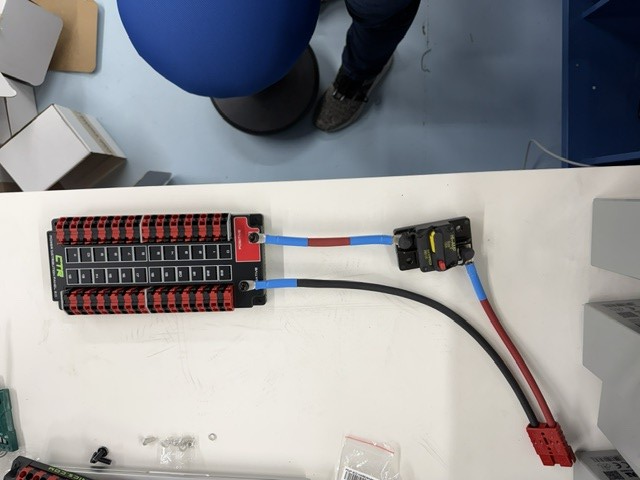
\includegraphics[width=0.85\textwidth]{media/image52.png}
\caption{The PDP wired with the 120A breaker and power cables.}
\end{figure}

Insert the
\href{https://store.ctr-electronics.com/products/power-distribution-panel-wago-tool?pr_prod_strat=jac\&pr_rec_id=6ce3ee740\&pr_rec_pid=7863766450349\&pr_ref_pid=8358474383533\&pr_seq=uniform}{WAGO}
tool or a sturdy flathead screwdriver into the square hole on the PDP
and tilting the tool upwards to release the clamp to install the power
cables for the motors and encoders in a row on the corresponding colors
on the PDP. Be sure that the cables are stripped 3/8'' on the end before
inserting into the panel. Next to each set of cables, install a 40A fuse
for the motors and the 10A fuse for the encoders.

\begin{figure}[H]
\centering
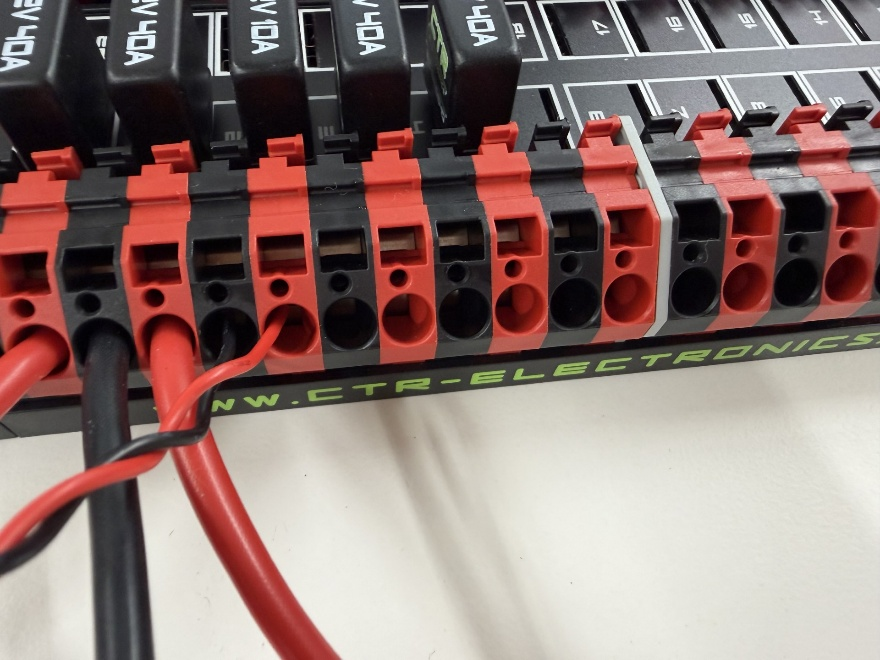
\includegraphics[width=0.47\textwidth]{media/image53.jpeg}
\hfill
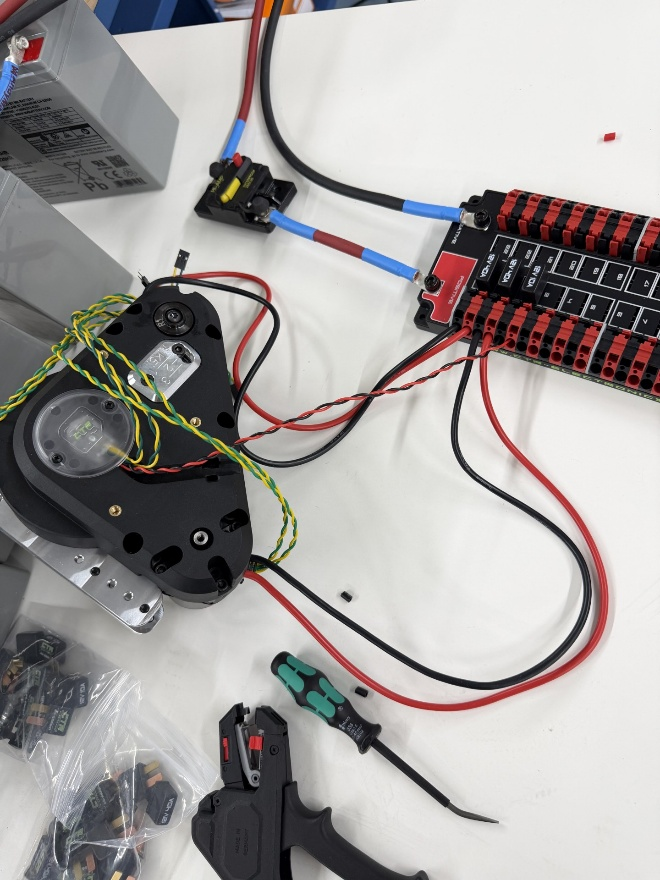
\includegraphics[width=0.47\textwidth]{media/image54.jpeg}
\caption{Installing the motor and encoder power cables with their 40A and
10A fuses.}
\end{figure}

Repeat for each Swerve Module assembly. Also install the 12'' battery
cables on the battery with the provided hardware.

\begin{figure}[H]
\centering
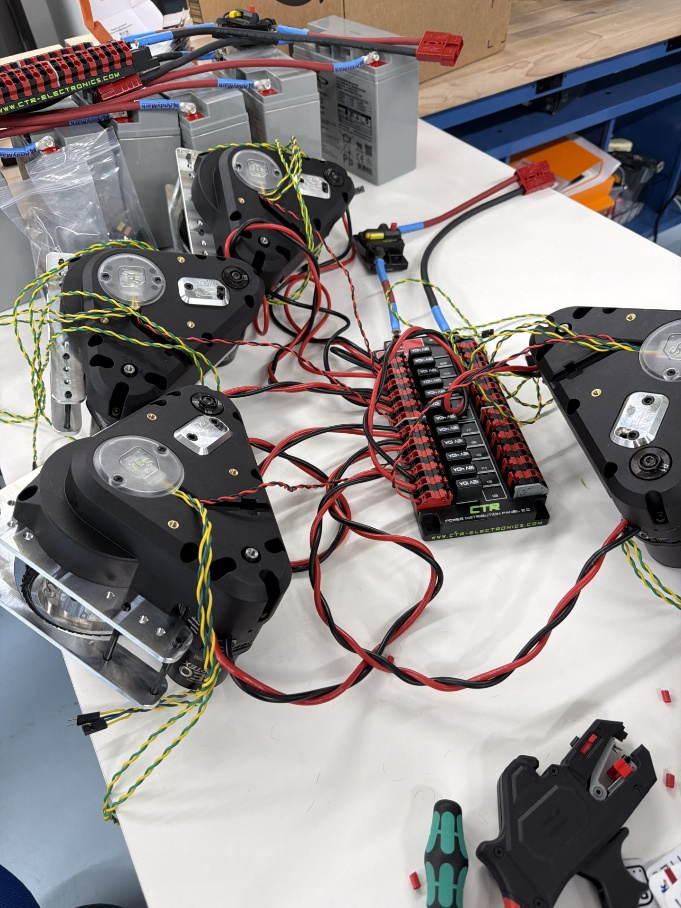
\includegraphics[width=0.5\textwidth]{media/image55.jpeg}
\caption{The 12'' battery cables attached to the battery terminals.}
\end{figure}
